
%%%%%%%%%%%%%%%%%%%%%%%%%%%%%%%%%%%%%%%%%%%%%%%%%%%%%%%%%%%%%%%%%%%%%%%%%%%%%%
% Copyright (c) 2003-2018 by The University of Queensland
% http://www.uq.edu.au
%
% Primary Business: Queensland, Australia
% Licensed under the Apache License, version 2.0
% http://www.apache.org/licenses/LICENSE-2.0
%
% Development until 2012 by Earth Systems Science Computational Center (ESSCC)
% Development 2012-2013 by School of Earth Sciences
% Development from 2014 by Centre for Geoscience Computing (GeoComp)
%
%%%%%%%%%%%%%%%%%%%%%%%%%%%%%%%%%%%%%%%%%%%%%%%%%%%%%%%%%%%%%%%%%%%%%%%%%%%%%%

\chapter{The \speckley Module}\label{chap:speckley}\index{speckley}
%\declaremodule{extension}{speckley}
%\modulesynopsis{Solving linear, steady partial differential equations using spectral elements}

{\it speckley} is a high-order form of {\it ripley}, supporting structured, 
uniform meshes in two and three dimensions. Uniform meshes allow a more regular 
division of elements among compute nodes. Possible orders range from 2 to 10,
inclusive.

{\it speckley} domains cannot be created by reading from a mesh file.

The family of domain that will result from a 
\class{Rectangle} or \class{Brick} call depends on which module is imported in
the specific script. The following line is an example of importing 
\speckley domains:

\begin{python}
 from esys.speckley import Rectangle, Brick
\end{python}

\section{Formulation}
For a single PDE that has a solution with a single component the linear PDE is
defined in the following form:
\begin{equation}\label{SPECKLEY.SINGLE.1}
\begin{array}{cl} &
\displaystyle{
\int_{\Omega}
D \cdot vu \; d\Omega } + \int_{\Gamma} d \cdot vu \; d{\Gamma}

= \displaystyle{\int_{\Omega}  X_{j} \cdot v_{,j}+ Y \cdot v \; d\Omega }
+ \displaystyle{\int_{\Gamma} y \cdot v \; d{\Gamma}}
\end{array}
\end{equation}

\section{Meshes}
\label{SPECKLEY MESHES}

\speckley meshes are formed of regular elements using Gauss-Labatto-Legendre
quadrature points. The number of quadrature points in each axis is dependent
on the order of the domain. Examples of small Rectangle domains of different 
orders are shown in Figure~\ref{SPECKLEY:FIG:MESHES}.

Meshfiles cannot be used to generate \speckley domains.

\begin{figure}
    \begin{center}
        \subfigure[order 3]{%
            \label{FIG:SPECKLEYMESH:ORDER3}
            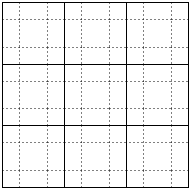
\includegraphics[width=0.3\textwidth]{speckley3}
        }%
        \subfigure[order 6]{%
            \label{FIG:SPECKLEYMESH:ORDER6}
            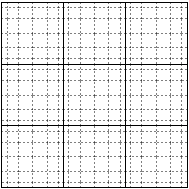
\includegraphics[width=0.3\textwidth]{speckley6}
        }%
        \subfigure[order 9]{%
            \label{FIG:SPECKLEYMESH:ORDER9}
            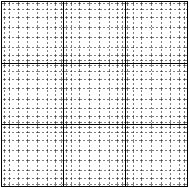
\includegraphics[width=0.3\textwidth]{speckley9}
        }%
    \end{center}
    \caption{3x3 \emph{speckley} Rectangle domains of different orders}
    \label{SPECKLEY:FIG:MESHES}
\end{figure}

\section{Linear Solvers in \SolverOptions}
While \speckley has the same defaults as \ripley, the \HRZLUMPING must be set.
\PASO is not used in \speckley.

\section{Cross-domain Interpolation}
Data on a \speckley domain can be interpolated to a matching \ripley domain
provided the two domains have identical dimension, length, and, in multi-process
situations, domain sub-divisions.

A utility class, \class{SpeckleyToRipley} is available to simplify meeting these
conditions. To gain access to the class, the following will be required in
the script:

\begin{python}
 from esys.escript.domainCouplers import SpeckleyToRipley
\end{python}

\section{Functions}
\begin{funcdesc}{Brick}{order,n0,n1,n2,l0=1.,l1=1.,l2=1.,d0=-1,d1=-1,d2=-1,
diracPoints=list(), diracTags=list()}
generates a \Domain object representing a three-dimensional brick between
$(0,0,0)$ and $(l0,l1,l2)$ with orthogonal faces. All elements will be regular
and of order \var{order}. The brick is filled with
\var{n0} elements along the $x_0$-axis,
\var{n1} elements along the $x_1$-axis and
\var{n2} elements along the $x_2$-axis.
If built with \MPI support, the domain will be subdivided 
\var{d0} times along the $x_0$-axis,
\var{d1} times along the $x_1$-axis, and
\var{d2} times along the $x_2$-axis.
\var{d0}, \var{d1}, and \var{d2} must be factors of the number of
\MPI processes requested.
If axial subdivisions are not specified, automatic domain subdivision will take
place. This may not be the most efficient construction and will likely result in
extra elements being added to ensure proper distribution of work. Any extra
elements added in this way will change the length of the domain proportionately.
\var{diracPoints} is a list of coordinate-tuples of points within the mesh,
each point tagged with the respective string within \var{diracTags}.
\end{funcdesc}

\begin{funcdesc}{Rectangle}{order,n0,n1,n2,l0=1.,l1=1.,l2=1.,d0=-1,d1=-1,d2=-1,
diracPoints=list(), diracTags=list()}
generates a \Domain object representing a two-dimensional rectangle between
$(0,0)$ and $(l0,l1)$ with orthogonal faces. All elements will be regular
and of order \var{order}. The rectangle is filled with
\var{n0} elements along the $x_0$-axis and
\var{n1} elements along the $x_1$-axis.
If built with \MPI support, the domain will be subdivided 
\var{d0} times along the $x_0$-axis and
\var{d1} times along the $x_1$-axis.
\var{d0} and \var{d1} must be factors of the number of \MPI processes requested.
If axial subdivisions are not specified, automatic domain subdivision will take
place. This may not be the most efficient construction and will likely result in
extra elements being added to ensure proper distribution of work. Any extra
elements added in this way will change the length of the domain proportionately.
\var{diracPoints} is a list of coordinate-tuples of points within the mesh,
each point tagged with the respective string within \var{diracTags}.
\end{funcdesc}
